% !TeX root = ../apuntes-ea.tex

\chapter{Grupos abelianos}

En este capítulo utilizamos notación aditiva, la habitual para hablar de grupos abelianos. Recordemos que además de escribir $a+b$ para la operación de dos elementos y $r\cdot a$ para denotar el elemento $a$ operado con sí mismo $r$ veces, escribiremos $G \oplus H$ para el producto directo (suma directa en este caso) y $G + H$ para el producto libre (suma libre en este caso).

\begin{dfn}[Suma directa]
	\label{dfn:sumadirecta}
	Sean $(G_1, +), \dots, (G_n, +)$ grupos (abelianos) cuya operación es la suma\footnote{Lo importante es que es la misma operación para todos y que utilizamos la notación aditiva, lo que \textit{suma} signifique en realidad nos importa poco} entonces denotamos por suma directa al producto directo de todos ellos:
	\begin{align*}
	\bigoplus_{i=1}^n (G_i, +) = \left(\bigoplus_{i=1}^n G_i, \oplus\right) = (G_1 \times \dots \times G_n, \oplus)
	\end{align*}
	donde $\oplus: (\bigoplus_{i=1}^n G_i) \times (\bigoplus_{i=1}^n G_i) \to \bigoplus_{i=1}^n G_i$ se define con $g \oplus g' = (g_1 + g'_1, \dots, g_n + g'_n)$.\footnote{Aquí el $\times$ que aparece se refiere al producto cartesiano, no al producto directo.}
\end{dfn}

Es importante no confundirlas en lo que sigue.

\begin{dfn}[\textit{Suma} libre de grupos]\footnote{Lo de suma libre me lo he inventado completamente.}
	\label{dfn:sumalibre}
	Sean $S,T$ subconjuntos del grupo $G$ (abeliano). Definimos $S+T = \{s+ t \mid s \in S \land t \in T\}$.
\end{dfn}

El objetivo de este capítulo es completar las proposiciones que teníamos sobre grupos abelianos para dar un teorema de clasificación válido para todo grupo abeliano finito. Con esto nos quitamos otra gran familia de grupos (ya nos habíamos quitado los cíclicos).

\section{Descomposición en suma directa}

\begin{pro}
	\label{pro:abelianosumadirecta}
	Sea $G$ un grupo abeliano, $H, K < G$. Entonces son equivalentes:
	\begin{enumerate}
		\item $H+K = G \land H \cap K = \{\0\}$
		\item \begin{align*}
			f:H\oplus K &\to G\\
			(h,k) &\mapsto h+k
		\end{align*}
		es un isomorfismo de grupos
	\end{enumerate}
\end{pro}

\begin{obs}
	Esta proposición también es cierta para 3 subgrupos (o más) siempre que cumplan que la intersección de un subgrupo con la suma libre de los demás sea nula:
	\begin{align*}
		K,H, N < G \text{ abeliano } \land H + K + N = G \land \begin{cases}
		H \cap (K+N) = \{\0\} \\
		K \cap (H+N) = \{\0\} \\
		N \cap (K+H) = \{\0\}
		\end{cases} \implies G \isom H \oplus K \oplus N
	\end{align*}
\end{obs}

Esto nos viene muy bien ya que los teoremas de Sylow justo nos proporcionan subgrupos cuya intersección es vacía: los p-grupos de Sylow, lo que nos lleva a una observación/teorema.

\begin{thm}
	Todo grupo abeliano es suma directa de sus p-subgrupos de Sylow.
\end{thm}

\begin{ej}
	Sea $G$ un grupo abeliano de orden $n = p_1^{\alpha_1}p_2^{\alpha_2}p_3^{\alpha_3}$. Por Sylow tenemos
	que $\exists P_1, P_2, P_3 < G$ tales que $|P_1| = p_1^{\alpha_1},\ |P_2| = p_2^{\alpha_2},\ |P_3| = p_3^{\alpha_3}$. Sabiendo que la intersección de subgrupos es un subgrupo y por tanto $|P_1 \cap P_2|$ tiene que dividir a $|P_1|$ y a $|P_2|$ que son primos tenemos que $|P_1\cap P_2| = 1 \implies P_1 \cap P_2 = \{\0\}$. Lo mismo ocurre con las demás combinaciones de p-subgrupos de Sylow por lo que concluímos que $G \isom P_1 \oplus P_2 \oplus P_3$.
\end{ej}

\begin{obs}
	Los elementos que viven en los p-subgrupos de Sylow son aquellos cuyo orden es una potencia de $p_i$:
	\begin{align*}
		P_i = \{g\in G \mid o(g)\text{ es una potencia de } p_i\}
	\end{align*}
\end{obs}

\begin{ej}
	Una manera de ver esto es definiendo para un $n \in \N$ fijo
	\begin{align*}
		G &\to G \\
		a &\mapsto n\cdot a
	\end{align*}
	tenemos que es un homomorfismo de grupos cuando $G$ es abeliano. En nuestro caso cogiendo $n = p_i^{\alpha_i}$ tenemos que $a \mapsto p_i^{\alpha_i} a = 0 \iff o(a) \divides p_i^{\alpha_i}$. Por ejemplo para $G = \Z/10\Z$ tenemos que $\exists P_2, P_5 < \Z/10\Z$ donde
	\begin{align*}
		P_2 &= \ker(\text{multiplicación por 2}) = \{\overline{0}, \overline{5}\} &\isom \Z/2\Z \\
		P_5 &= \ker(\text{multiplicación por 5}) = \{\overline{0}, \overline{2}, \overline{4}, \overline{6}, \overline{8}\} &\isom \Z/5\Z
	\end{align*}
	Y se dan las hipótesis de la \autoref{pro:abelianosumadirecta} por lo que concluímos que $\Z/10\Z = P_2 \oplus P_5 \isom \Z/2\Z \oplus \Z/5\Z$
\end{ej}

\begin{ej}
	Consideramos $G = \Z/12\Z$. Por Sylow tenemos $\exists P_2, P_3 < \Z/12\Z$ tales que
	\begin{align*}
		P_2 &= \{\overline{0}, \overline{3}, \overline{6}, \overline{9}\} &= \text{elementos cuyos órdenes son potencia de } 2 &\isom \Z/4\Z\\
		P_3 &= \{\overline{0}, \overline{4}, \overline{8}\} &= \text{elementos cuyos órdenes son una potencia de } 3 &\isom \Z/3\Z
	\end{align*}
	Y por tanto $\Z/12\Z \isom P_2 \oplus P_3 \isom \Z/4\Z \oplus \Z/3\Z$.
\end{ej}

\begin{obs}
	Esta descomposición es unívoca (salvo reordenaciones de los sumandos): en grupos abelianos los p-subgrupos de Sylow son únicos ya que al ser todos normales los $n_i = 1$.
\end{obs}

\section{P-grupos abelianos finitos}

\begin{wrapfigure}{l}{0.4\textwidth}
	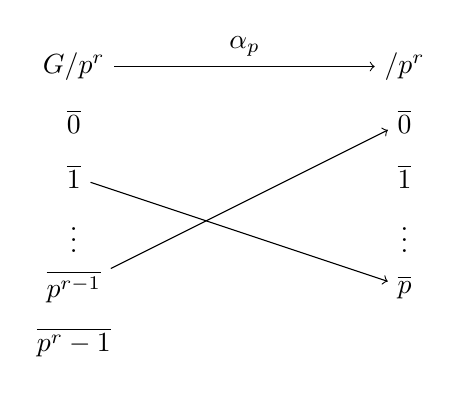
\begin{tikzpicture}
	\begin{scope}[scale=.7]
	\node (G) at (0,4) {$G \isom \Z/p^r\Z$};
	\node (G2) at (6,4) {$\Z/p^r\Z$};
	\node (0) at (0,3) {$\overline{0}$};
	\node (0b) at (6,3) {$\overline{0}$};
	\node (1) at (0,2) {$\overline{1}$};
	\node (1b) at (6,2) {$\overline{1}$};
	\node (dots) at (0,1) {$\vdots$};
	\node (dots2) at (6,1) {$\vdots$};
	\node (p1) at (6,0) {$\overline{p}$};
	\node (prm1) at (0,0) {$\overline{p^{r-1}}$};
	\node (pr) at (0,-1) {$\overline{p^r - 1}$};
	\draw[->] (G) -- (G2) node[above, pos=.5] {$\alpha_p$};
	\draw[->] (1) -- (p1);
	\draw[->] (prm1) -- (0b);
	\end{scope}
	
	\end{tikzpicture}
	\caption{El homomorfismo de grupos $\alpha_p$.}
	\label{fig:homomorfismoalphap}
\end{wrapfigure}

Sea $G$ un grupo abeliano con $|G| = p^r,\ r \in \N \implies \forall g \in G,\ o(g) = p^s$ con $s \leq r$. Recordemos que si $n \in \Z$ la función $\alpha_n :G \to G,\ a \mapsto n\cdot a$ es un homomorfismo de grupos cuando $G$ es abeliano.

Para este caso nos interesa tomar $n = p$ y observar que $\alpha_p(a) = p\cdot a$ no es inyectiva por ser $|G| = p^r$.
% TODO por qué?


\begin{pro}
	El homomorfismo de grupos $\alpha_p:G \to G$ para un $G$ p-grupo abeliano finito tiene núcleo no trivial. Es decir, $\{\0\} \subsetneq \ker \alpha_p < G$
\end{pro}

\begin{proof}
	 Por el \autoref{thm:lagrange} $|G| = n \land p \divides n \implies \exists \alpha \in G \mid o(\alpha) = p$ (aquí $p$ es primo). De modo que 
	 \begin{align*}
	 	\ker \alpha_p = \{g \in G \mid o(g) \divides p \} \supset \{0, \alpha \mid o(\alpha) = p\} \supsetneq \{\0\}
	 \end{align*}
\end{proof}

\begin{obs}El elemento $p^{r-1}$ tiene orden $p$ y genera el único subgrupo de orden $p$.
\end{obs}

\begin{obs}
	$\ima \alpha_p = \gen{\alpha(\overline{1})} = \gen{\overline{p}} \isom \Z/p^{r-1}\Z$.
\end{obs}

Si ahora consideramos $G \isom \Z/p^r\Z \oplus \Z/p^s\Z$ (que no es cíclico porque $mcd(p^r, p^s) \geq p > 1$) veamos que lo anterior no se cumple. Sean $\overline{a} \in \Z/p^r\Z,\ \overline{\overline{b}} \in \Z/p^s\Z$.

\begin{align*}
	\alpha_p : G &\to G \\
	(\overline{a}, \overline{\overline{b}}) &\mapsto (p\overline{a}, p\overline{\overline{b}}) \\
\end{align*}
\begin{align*}
	\ker \alpha_p = \{(\overline{a}, \overline{\overline{b}}) \in G \mid p \overline{a} = \0 \land p\overline{\overline{b}} = \0\} \\
	\ker \alpha_p = \gen{\overline{p^{r-1}}} \oplus \gen{\overline{p^{s-1}}} \isom \Z/p\Z \oplus \Z/p\Z
\end{align*}

En este caso, hay más de un subgrupo de orden $p$. Por ejemplo
\begin{align*}
	\gen{(\overline{0}, \overline{1})} &\subset \Z/p\Z \oplus \Z/p\Z\text{ y tiene orden } p \\
	\gen{(\overline{1}, \overline{0})} &\subset \Z/p\Z \oplus \Z/p\Z\text{ y tiene orden } p
\end{align*}
Esta lista no es exhaustiva, hay más...

\section{Teorema de estructura de grupos abelianos finitos}

Previamente a dar el teorema gordo, veremos algunos resultados.

\begin{pro}
	Sea $G$ un p-grupo abeliano. Entonces $G$ es cíclcio $\iff$ tiene un único subgrupo de orden $p$.
\end{pro}

\begin{proof}
	Pendiente de los apuntes de Santorum página 146 % TODO
\end{proof}

\begin{pro}
	Sea $G$ un p-grupo abeliano con $|G| = p^r$. Sea $L$ un subgrupo cíclico de orden máximo\footnote{Esto significa que $|L|$ es el mayor divisor de $|G|$ para el que $L$ es cíclcio. Se tendrá que si $G$ ya es cíclico entonces $L = G$ y $H = \{\0\}$.} en $G$. Entonces $\exists H < G$ tal que $G \isom L \oplus H$.
\end{pro}

\begin{proof}
	Santorum pág 197 % TODO
\end{proof}

\begin{pro}[de estructura de p-grupos abelianos]
	Sea $G$ un p-grupo abeliano finito. Entonces $G$ es suma directa de subgrupos cíclicos:
	\begin{align}
		G \isom L_1 \oplus L_2 \oplus \dots \oplus L_q,\qquad L_i < G\text{ cíclico }
	\end{align}
\end{pro}

\begin{cor}
	Si $L_i = \Z/p_i\Z$ y reordenamos los índices para obtener
	\begin{align}
		\label{eq:secuenciaintrinseca}
		p^{r_1} \geq p^{r_2} \geq \dots \geq p^{r_q}
	\end{align}
	entonces la secuencia \ref{eq:secuenciaintrinseca} es intrínseca a $G$.
\end{cor}

\begin{proof}
	Santorum pág 149
\end{proof}

\begin{dfn}[Expresión característica]
	Sea $G$ un p-grupo abeliano que se descompone en $G \isom L_1 \oplus \dots \oplus L_q$ con $L_i \isom \Z/p^{r_i}\Z$. La expresión característica de $G$ es la desigualdad que resulta de reordenar los índices para que se cumpla
	\begin{align}
		\label{eq:eqcaracteristica}
		p^{r_1} \geq p^{r_2} \geq \dots \geq p^{r_q}
	\end{align}
\end{dfn}

\begin{ej}
	Sea $G = \uds{\Z/12\Z} = (\{\overline{1}, \overline{5}, \overline{7}, \overline{11}\}, \cdot)$. Observemos que $G$ contiene 3 elementos de orden 2. Esto nos recuerda a una presentación de $\Z/2\Z \oplus \Z/2\Z$ y concluimos que $G \isom \Z/2\Z \oplus \Z/2\Z$ y por tanto la expresión característica es $2^1 \geq 2^1$.
\end{ej}

\begin{ej}
	Sea $G = \uds{\Z/60\Z}$. Se pide comprobar que $G$ es un $p$-grupo y dar su expresión característica.
\end{ej}

\begin{proof}[Solución]
	Observemos que $\Z/60\Z \isom \Z/12\Z \oplus \Z/5\Z$ ya que $mcd(12, 5) = 1$ y observemos que\footnote{Aquí estamos medio adelantando la \autoref{pro:udsproductodirectoanillos} que se probará cuando se introduzcan formalmente las unidades que son un concepto de anillos.}
	\begin{align*}
		\uds{\Z/60\Z} &= \{(a,b) \in \Z/60\Z \mid o(a) = 12 \land o(b) = 5\} \\
		a &\in \uds{\Z/12\Z} = \{\overline{1}, \overline{5}, \overline{7}, \overline{11}\} \isom \Z/2\Z \oplus \Z/2\Z \\
		b &\in \uds{\Z/5\Z} = \{\overline{1}, \overline{2}, \overline{3}, \overline{4}\} \isom \Z/4\Z \\
		\implies& \uds{\Z/60\Z} = \Z/2\Z \oplus \Z/2\Z \oplus \Z/4\Z
	\end{align*}
	y por tanto la secuencia asociada es $2^2 \geq 2^1 \geq 2^1$.
\end{proof}

Con esto y sabiendo que la descomposición en p-grupos de un grupo abeliano es única estamos a nada de enunciar el teorema de estructura pero antes veamos un ejemplo de aplicación de los resultados anteriores.

\begin{ej}
	Sea $G = \Z/p\Z \oplus \Z/p\Z$. Nos preguntamos cuántos subgrupos de orden $p$ contiene $G$.
\end{ej}

\begin{proof}[Solución]
	Observemos que $|G| = p^2$ y que los elementos de $G$ solo pueden tener orden 1 u orden $p$. Es decir que en $G$ hay
	\begin{align*}
		p^2-1 &\text{ elementos de orden } p \\
		1 &\text{ elemento de orden } 1 \text{ (el neutro) }
	\end{align*}
	Por tanto tenemos que $\forall a \in G,\ \0 \neq a$ hay un $H < G,\ H = \gen{a}$ con $|H| = p$. Además $H$ contiene 1 elemento de orden 1 (el neutro) y $p-1$ elementos de orden $p$. Además, recordemos que los elementos $a$ de orden $p$ solo pertenecen a uno de los subgrupos $H$ ya que en cuanto pertenezcan a dos, los dos subgrupos son necesariamente el mismo. Por tanto el número de subgrupos de orden $p$ se obtiene de repartir los elementos de orden $p$:
	\begin{align*}
		 \frac{p^2-1}{p-1} = \frac{(p-1)(p+1)}{(p-1)} = p+1 \text{ subgrupos de orden } p
	\end{align*}
\end{proof}

\begin{thm}[de estructura de grupos abelianos finitos]
	Todo grupo abeliano es isomorfo a una suma directa de p-grupos cíclicos. 
\end{thm}